\ctable[caption={Studying a problem at multiple scales},
		label={fig:scales},
		figure]{c}{\tnote[]{}}{\FL
			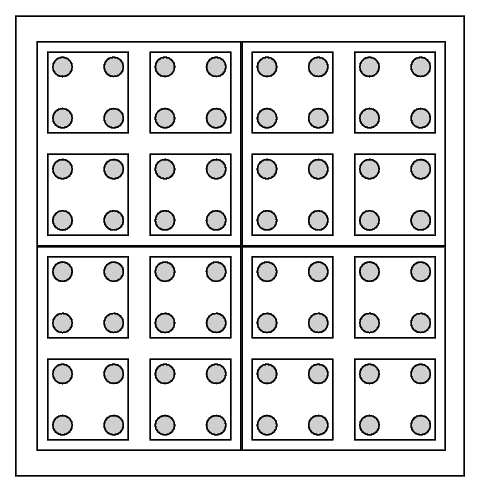
\includegraphics[scale=0.2]{fig/ising.png}
		\LL}
The heart of our method for solving the TSP problem is the renormalization
theory. The renormalization theory is originating from theoretical physics. In
theoretical physics renormalization is used to study the observe the changes
in a physical system. The changes are observed by looking to the problem at
different scales. This idea is illustrated in figure \ref{fig:scales}.


This idea is mapped onto the Traveling Salesman problem. The total square in
figure \ref{fig:scales} can be seen as the total area where the cities are
located. When estimating the shortest route, we start at a large scale, and we
keep zooming in until our estimated path visiting all cities is known. The
procedure is illustrated in figure 
%\ref{fig:renormalization}. 
The image on the
topleft of the figure is the basic block. This basic block consists of four
cells. A cell represents a virtual city, available if one or more cities are
within the cell. The general idea of the algorithm is to solve the Traveling
Salesman problem for the larger block. This can be done easily, because a
Traveling Salesman problem for at most four cities can be easily solved, by
simply enumerating all possibilities. Then this block can be divided into four
subblocks. Together with some information acquired from the larger block, the
Traveling Salesman problem can again be solved for the four subblocks. This
process is repeated until there is at most one city in a cell, and the
estimated route is known. In the following subsection we will describes the
steps in the algorithm in more detail.

\subsection{Preprocessing step}
\ctable[caption={The basic two by two cell},
	label={fig:basiccell},
	figure]{c}{\tnote[]{The open circles are the border points, the closed circles
		are the centre of the cells and the crosses are additional places where an
		edge crosses the border of a cell}}{\FL
	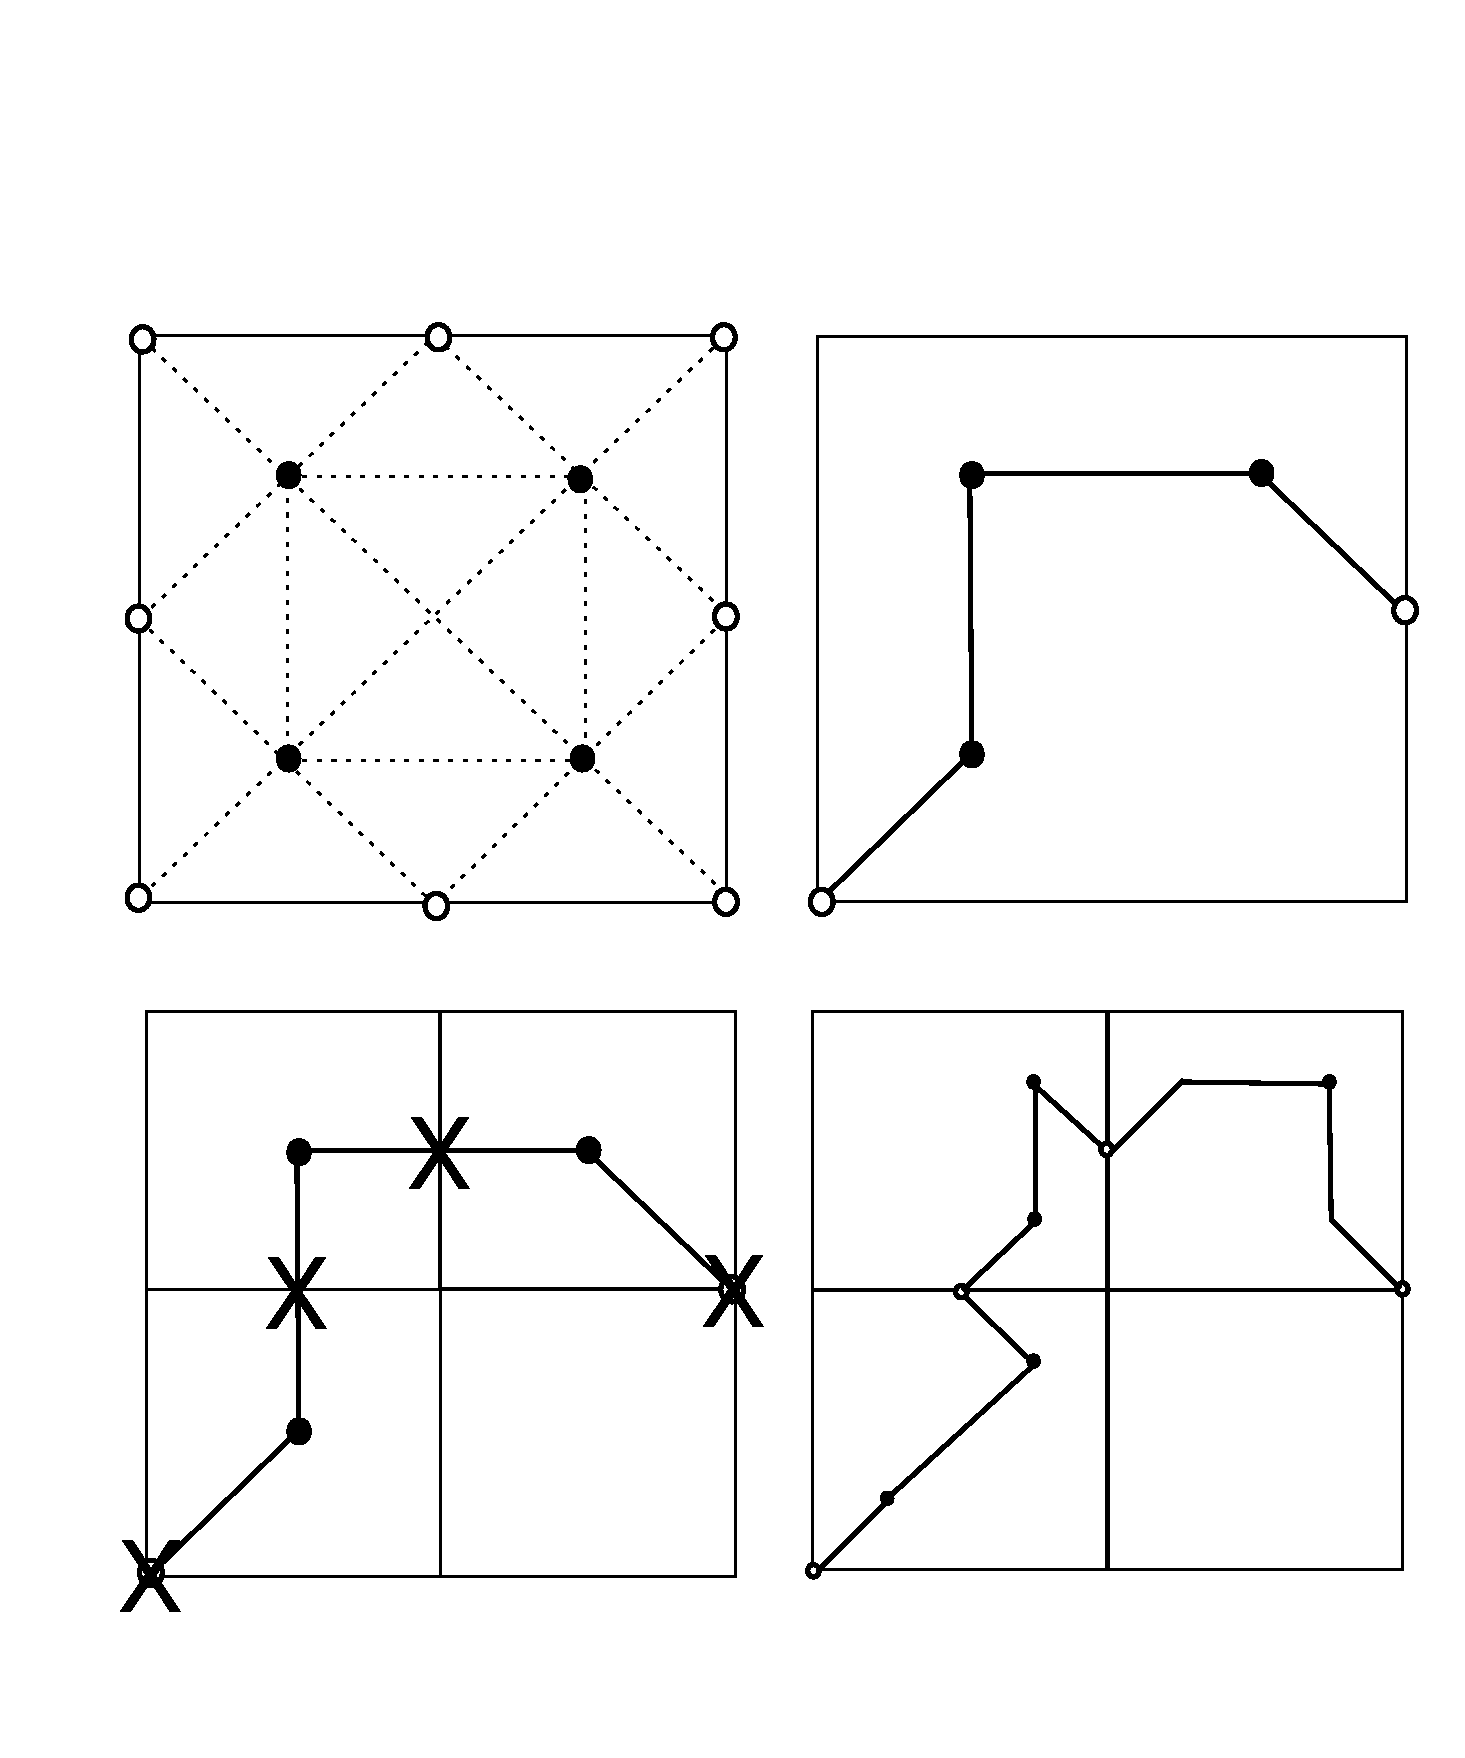
\includegraphics[width=7cm]{fig/renormalization.pdf}
	\LL}

The preprocessing step prevents the performance penalty each time you need to
calculate an optimal route in a block. Basically this means that for every
possible configuration you calculate the optimal path. There are two aspects
which can be altered, the border point at which the route is started and the
visited cells.

For retrieving the shortest route through a block, it is considered as a
graph. The nodes are the border points and the cell points (Lying in the
centrum of a cell). The nodes are connected by multiple Before treating on the
algorithm the preprocessing is considered.  The preprocessing consists of
calculating all shortest paths in the basic blocks. Here all possible subsets
of cells that needs to be visited are considered.

The basic block can be treated as a graph, the border points and the cell
points are the nodes. There are edges between the border points and their
closest cell point(s). The cell points are also connected with an edge with
the other cell points. This set-up can be seen in the topleft picture of
figure %\ref{fig:renormalization}. 
For getting the shortest route, a breadth
first search is used. Here all possible paths, without cycles, between the
starting and end node are calculated. Using these set of paths, the shortest
routes visiting subsets of cell points are searched.

\subsection{First iteration}
\subsection{Further iterations}
\subsection{Retrieving the estimate of the shortest tour}

\ctable[caption={The first four iterations on d198.tsp},
		label={fig:iterations},
		width=7.5cm,
		figure]{cc}{\tnote[]{Some comments}}{\FL
			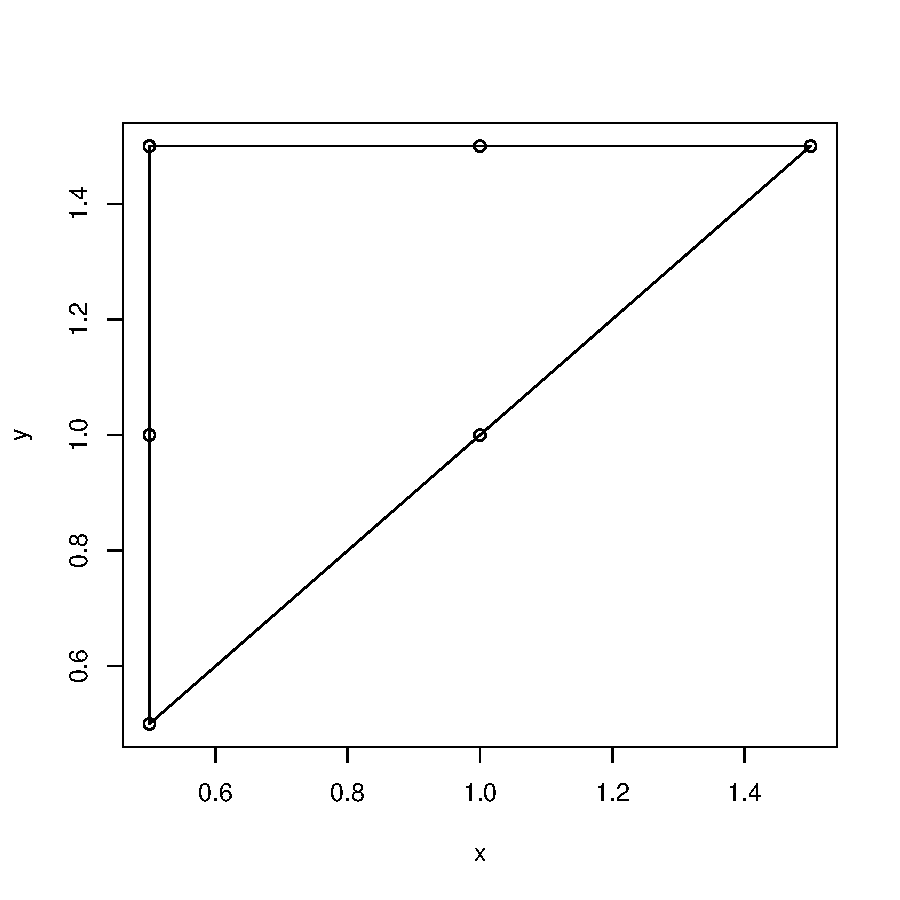
\includegraphics[width=3.5cm]{fig/it2.pdf} &
			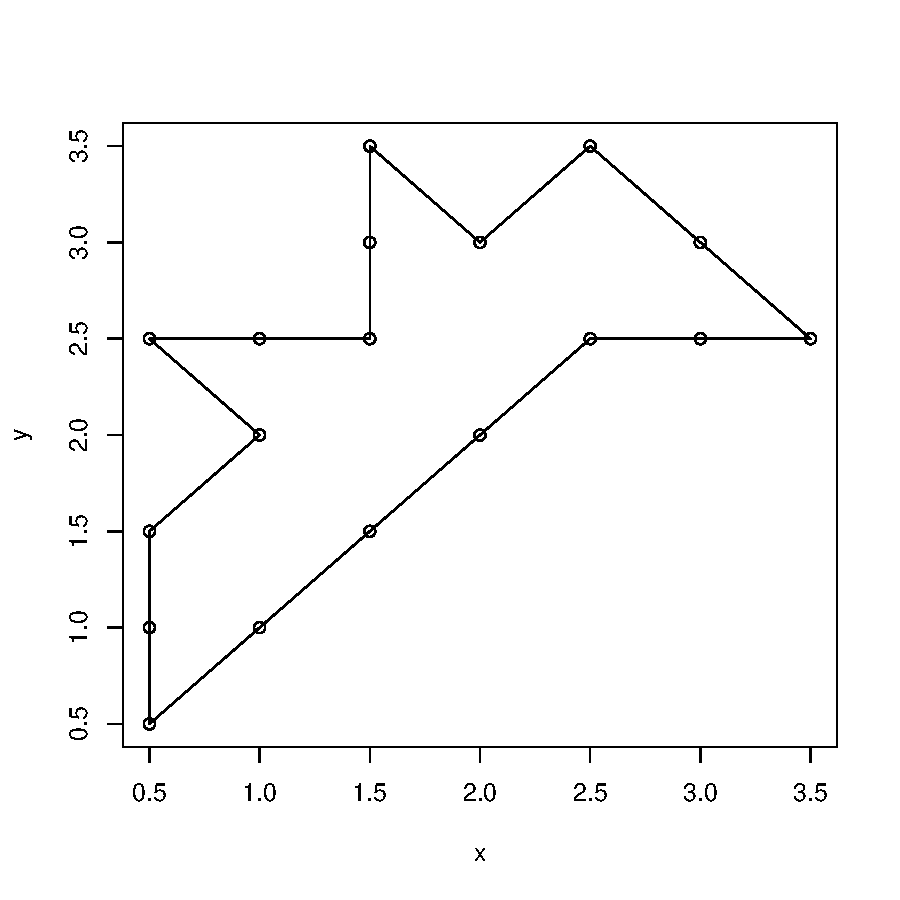
\includegraphics[width=3.5cm]{fig/it4.pdf} \NN
			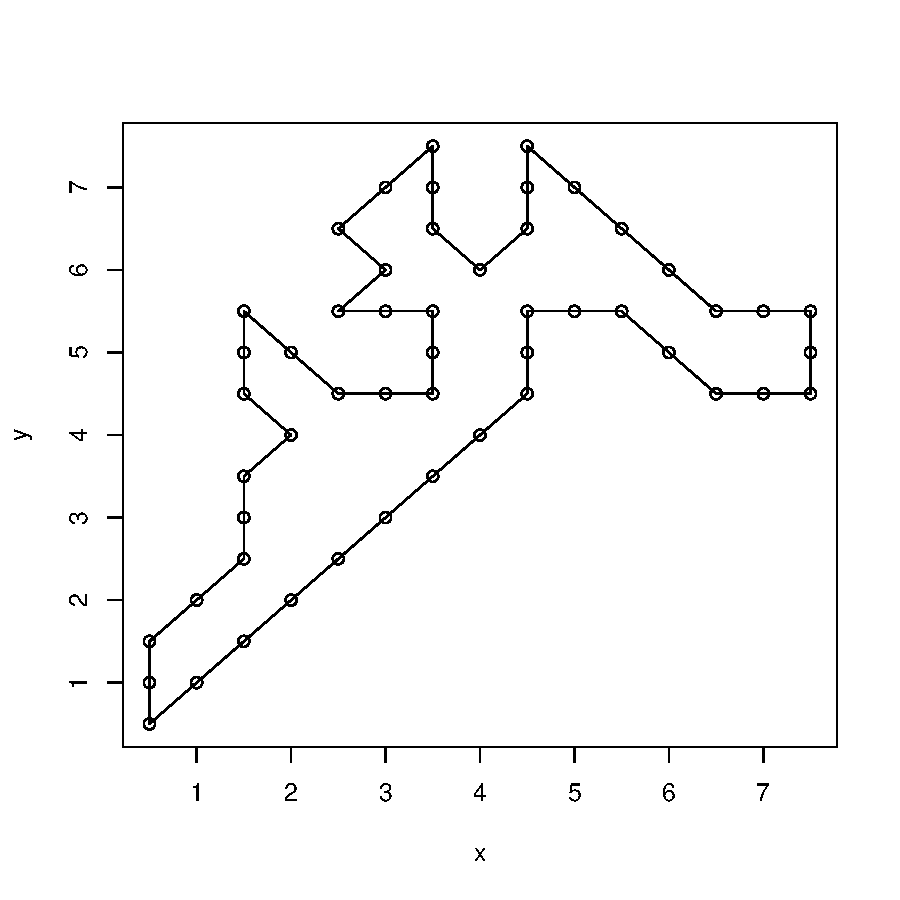
\includegraphics[width=3.5cm]{fig/it8.pdf} &
			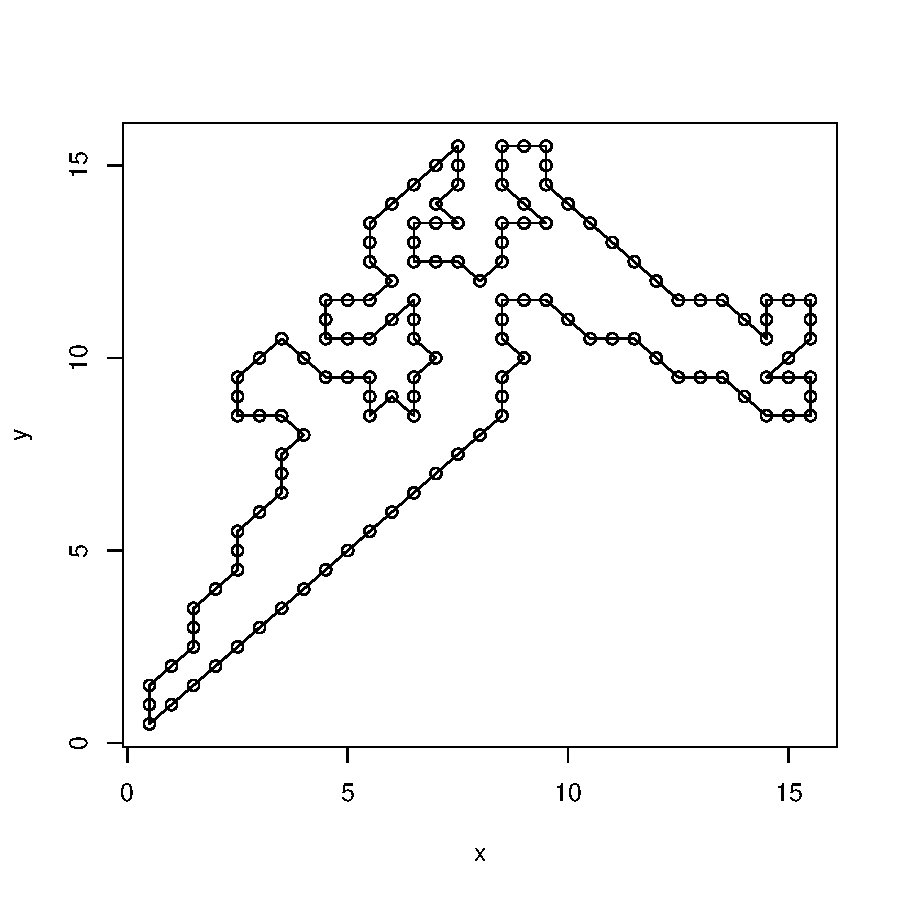
\includegraphics[width=3.5cm]{fig/it16.pdf} 
			\LL}

For finding the shortest route we do not treat all cities independently, but
we first try to solve the problem at the largest scale. For doing this we
divide the square into a block of a two by two cells. Within these cells we
take the average behavior. In case of the Traveling Salesman problem, we look
if there is a city within the cell or not. Now we decide the shortest route
for this two by two cell which visits all the cells where a city is located.

This basic two by two cell can be seen in figure \ref{fig:basiccell}. We
still need to solve the Traveling Salesman Problem on this smaller block. This
block however, is small enough to compute the shortest path with reasonable
performance. The renormalization method, needs to solve the TSP on this basic
cells repeatedly. For that reason all possible shortest paths are
precalculated. This means that from every possible route through the basic
block, the shortest path is calculated. This shortest path is calculated for
every possible combination of cells which needs to be visited.

When we solved the problem at a specific scale, we zoom in further. This means
that the blocks used in the current scale are divide in four subblocks, each
consist four cells. The route which we calculated in the previous block, can
now be used for calculating the shortest path through each of these subblocks.
For this we determine the cross points of the used edges in the shortest route

Renormalization Theory is a deterministic approach to solving the TSP problem.
The renormalization theory is originating from theoretical physics. In
theoretical physics renormalization theory is used for investigating the
changes of a physical system, by viewing it at different scales.

When we are applying renormalization theory to the TSP problem, we first solve
the TSP at a large scale. This solution is used recursively to solve it a
smaller scale. This is repeated until the scale is small enough for retrieving
a hamiltonian path connecting all cities.

Now we summerarized the method, we go more into detail. The solving process is
started by calculating the shortest path for a two by two block...

% vim:ft=tex:spell spelllang=en:autoindent
